
%%----------------------------------------------------------------------
 
\documentclass[a4paper,twoside]{IEEEtran}


\usepackage[%
               psphotos,      % uncomment those options you want
               photofit,%
        %       PStimes,%
        ]{ieeepes}


\usepackage{filecontents}
\begin{filecontents*}{bib.bib}

@REPORT{1,author={Mustafa S. Al-Ghafli},title={{Programming sirit 610 notes}}, year={2012}}
@REPORT{2,author={Yazan Hlayel, Mohammad Makkawi, Rami Rustom, Turki Al-Mutawa},title={{Handicapped Parking Project for COE 424}}, year={2014}}

\end{filecontents*}


\title{Bus Tracking and Monitoring System Using RFID Technology}

\author{
        Mosab Wadea\\
        201021320
\and
        Omar Amin\\
        201073280
\and
        Ahmed Bajubair\\
        201152850
\and
        Mahdi Sahel\\
        201152070
}


\usepackage{Pgfplots}


\usepackage{graphicx}
\usepackage{color}
\usepackage{courier}
\definecolor{bluekeywords}{rgb}{0,0,1}
\definecolor{greencomments}{rgb}{0,0.5,0}
\definecolor{redstrings}{rgb}{0.64,0.08,0.08}
\definecolor{xmlcomments}{rgb}{0.5,0.5,0.5}
\definecolor{types}{rgb}{0.17,0.57,0.68}

\usepackage{listings}
\lstset{language=[Sharp]C,
captionpos=b,
frame=l,
showspaces=false,
showtabs=false,
breaklines=true,
showstringspaces=false,
breakatwhitespace=true,
escapeinside={(*@}{@*)},
commentstyle=\color{greencomments},
morekeywords={partial, var, value, get, set},
keywordstyle=\color{bluekeywords},
stringstyle=\color{redstrings},
basicstyle=\ttfamily\small,
}
\usepackage{varioref}

\begin{document}

\maketitle


\begin{abstract}
This paper deals with designing and implementation of an RFID monitoring system for KFUPM transportation department. The overall system consist of a network of devices connected together and managed by a computer system. The system collects data from readers and process the data to present it to the users as useful information about the bus system status and availability of busses.
\end{abstract}


%beginning sections
\section{Introduction}
Add introduction
Add introduction
Add introduction
Add introduction
Add introduction


Add introduction
Add introduction
Add introduction
Add introduction
Add introduction
Add introduction
Add introduction
Add introduction



Add introduction
Add introduction
Add introduction
Add introduction
Add introduction
Add introduction
Add introduction


Add introduction
Add introduction
Add introduction
Add introduction
Add introduction
Add introduction
Add introduction
Add introductionAdd introduction
%%%%%%
%%%%%%
\section{Problem}
The main transportation method in KFUPM is the bus system that is supervised and ran by the transportation department. The problem with the system depends on the knowledge of the student about the timing of the busses movements and when busses are located in any station. If a small delay or error happens in the system it will affect all the time schedule and the flow of the busses. This error is most likely to occur and can not be prevented. The problem with the students is that they will not be able to identify when a delay occurs and wither a bus is available or not.

%%%%%%%
%%%%%%%
\section{Solution}
The solution proposed in this project is to provide a monitoring system for both the student and the administrators. Where students can access a website to check for busses and their availability, as will as the administrators who can view the tracking results and evaluate the efficiency of the system.
%%%%
\subsection{Requirements}
In order for the project to fulfill the needs it must sustain the following requirements:
\begin{itemize}
\item
Identify the busses and their assigned lines.
\item
Detect the busses and their movements.
\item
Detect busses on the run without the need to stop.
\item
Users can interact with the system and submit complaints.
\item
Administrators can access the system to evaluate the efficiency.
\item
Ability to accommodate multiple lines.
\end{itemize}
%%%%
\subsection{Specifications}
In order to make these requirements feasible the project has to implement the following specifications:
\begin{itemize}
\item 
Attach RFID passive tag to each bus.
\item
Install RFID reader and antenna at each bus station.
\item
Develop web based application that connects to the readers and fitch data and displays them.
\end{itemize}


%%%%%
%%%%%
\section{Project Design}
The system will depend on the bus stations as scanning locations for the busses. Each bus is tagged with an RFID passive tag. These tag are identified in the system by their unique ID (UID). When the bus approaches a bus station it will check into that station. This will let the system know when the bus is checked in and it will know what is the estimated time of arrival (ETA) to the next station. The users can access all these information from the web-base front-end interface. In \figref{blockdiagram} the block diagram shows how the components of the system are integrated together.
%%%
\subsection{Block diagram}
In the block diagram seen in \figref{blockdiagram} there are three main components that interact with the system, the bus station which contains the readers and the antennas, the front-end that consists of the students interface and the administrators panel, the last component is the bus that is tagged with an RFID tag. All these components are linked together and processed in the server. The server contains the software that will be described in details in the next section.
\begin{figure}
\centering
\fbox{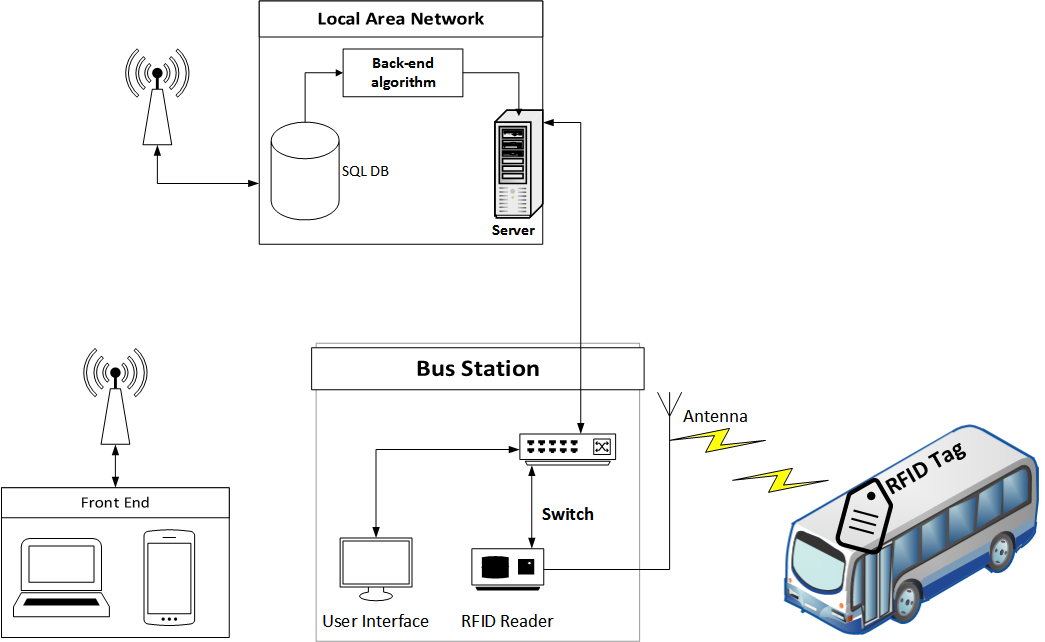
\includegraphics[scale=0.9]{blockdiagram/hardware.png}}
\caption{The block diagram of the system}
\label{blockdiagram}
\end{figure}
%%%
\subsection{Software architecture}
The software part is divided into three main parts as shown in \figref{blockdiagram} in the local area network tear, these three main parts are:
\begin{itemize}
\item
Back-end logic.
\item
The database.
\item
Web server.
\end{itemize}
The back-end contains a script that will communicate with the reader to check the busses availability at each station and it will write these information to a database. The web server will communicate with the database to get the latest information and it will update the front-end interface without the need to refresh the page by the user. The database is constructed of the following tables:
\begin{itemize}
\item
Bus.
\item
Path.
\item
Line.
\item
Station.
\item
Lo
\end{itemize}
The entity model shown in \figref{entity} shows the database structure and the attributes for each entity.
\begin{figure}
\centering
\fbox{\includegraphics[scale=1.2]{blockdiagram/entity.png}}
\caption{The entity model of the database}
\label{entity}
\end{figure}
%%%%%%%%
%%%%%%%%
\section{Methodology}
The system is divided into two main parts, software and hardware. The software will contain the database as well as the communication with the reader as part of the back-end and the front-end which is the website of the service. The hardware consists mainly from the reader and the antennas as well as the tags attached to each bus.
%%%%%%
\subsection{Hardware}
A selection of appropriate hardware was made to match all the requirements of the project, here is a brief description for each hardware part and how it is tested and implemented:
\begin{figure}[h]
\centering
\fbox{\includegraphics[scale=0.055]{img/img_20150515_172325.jpg}}
\caption{The sirit RFID reader and the antennas connected}
\label{sirireader}
\end{figure}
\subsubsection{Sirit RFID reader}
The sirit RFID reader has three interfacing methods: by GPIO, Serial and by network connection. This project will use the network approach since the bus stations are going to be located remotely and the most reliable way is by ethernet connection. This reader has a documentation \cite{1} that was used. The device can be configured to read from different antennas and it can return the number of antenna that detected a tag and the tag ID. In \figref{sirireader} it is shown the reader and three antennas that were connected to it. 
\subsubsection{RFID antenna}
The antenna used can work with power up to 300 watt and they are sensitive to the orientation. Some tests were made to find the optimum power and orientation of the antenna, and they are as follows:
\begin{description}
\item[Test1] 
this test was made with the antenna places on a height of 1.1 meter and oriented vertically, the distance between the tag and the antenna is 2.5 meters. the readings in \figref{read1} were collected in read time of 300 ms.
\begin{figure}[ht]
\centering
\fbox{
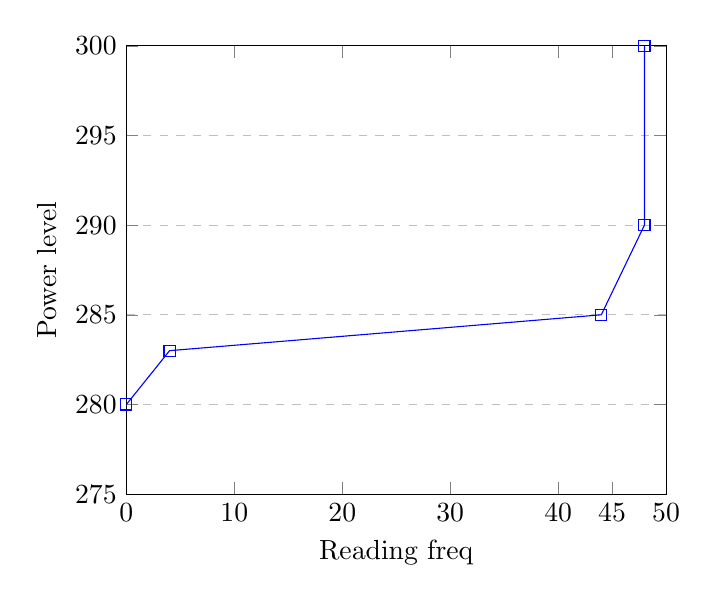
\begin{tikzpicture}
\begin{axis}[
    xlabel={Reading freq},
    ylabel={Power level},
    xmin=0, xmax=50,
    ymin=275, ymax=300,
    xtick={0,10,20,30,40,45,50},
    ytick={275,280,285,290,295,300},
    ymajorgrids=true,
    grid style=dashed
]
\addplot[
    color=blue,
    mark=square,
    ]
    coordinates {
    (48,300)(48,290)(44,285)(4,283)(0,280)
    };
\end{axis}
\end{tikzpicture}}
\caption{Results for test 1}
\label{read1}
\end{figure}
\\
\\
\\
\item[Test2] 
this test was made with the antenna places on a height of 2.1 meter and oriented horizontally, the distance between the tag and the antenna is 2.5 meters. the readings in \figref{read2} were collected in read time of 300 ms.
\begin{figure}[h]
\centering
\fbox{
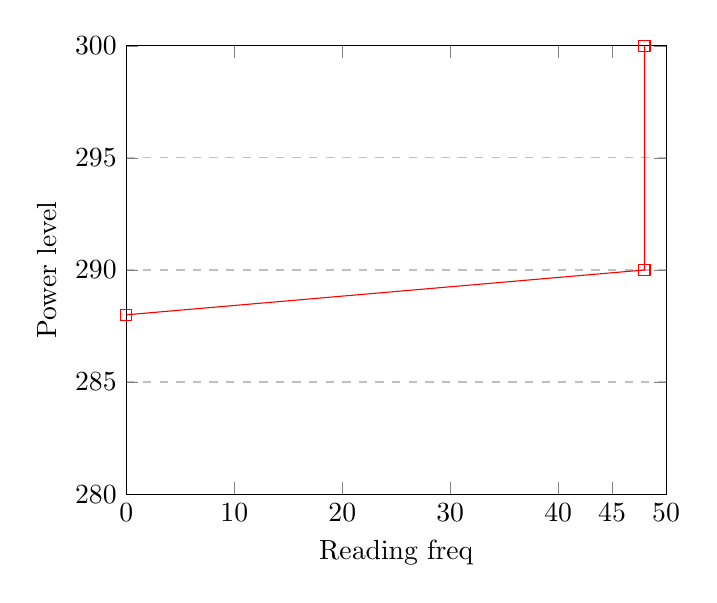
\begin{tikzpicture}
\begin{axis}[
    xlabel={Reading freq},
    ylabel={Power level},
    xmin=0, xmax=50,
    ymin=280, ymax=300,
    xtick={50,45,40,30,20,10,0},
    ytick={280,285,290,295,300},
    ymajorgrids=true,
    grid style=dashed,
]
 
\addplot[
    color=red,
    mark=square,
    ]
    coordinates {
    (48,300)(48,290)(0,288)
    };
\end{axis}
\end{tikzpicture}}
\caption{Results for test 2}
\label{read2}
\end{figure}

\end{description}
These tests shows that there will be huge drop in reading efficiency when the power goes below 280, but it will be approximately the same from 290 to 300. Therefor the power setting for the antenna is going to be 290 watt with horizontal orientation since this orientation allowed the antenna to be higher, and this is useful since the antenna must be placed over the bus stations. \figref{antenna} shows the antenna and how they are oriented.
\begin{figure}[h]
\centering
\fbox{\includegraphics[scale=0.2]{img/img_20150515_172358.jpg}}
\caption{Antenna oriented horizontally}
\label{antenna}
\end{figure}
\subsubsection{RFID tags}
The tags used are passive ultra high frequency (UHF) tags with programmable UID. The system will assign a tag to each bus and it will link the tag number with the bus number in the database. In \figref{tag} a sample of the tag used. This tag can handle the rough environment conditions such as high temperature, dust and collisions.
The specifications of this kind of tags are\cite{2}:
\begin{itemize}
\item
UHF tag (865-928) MHz.
\item
64 Bytes memory.
\item
Works in high temperature.
\item
Orientation-independent.
\item
Works with/around metal.
\end{itemize}
\begin{figure}[h]
\centering
\fbox{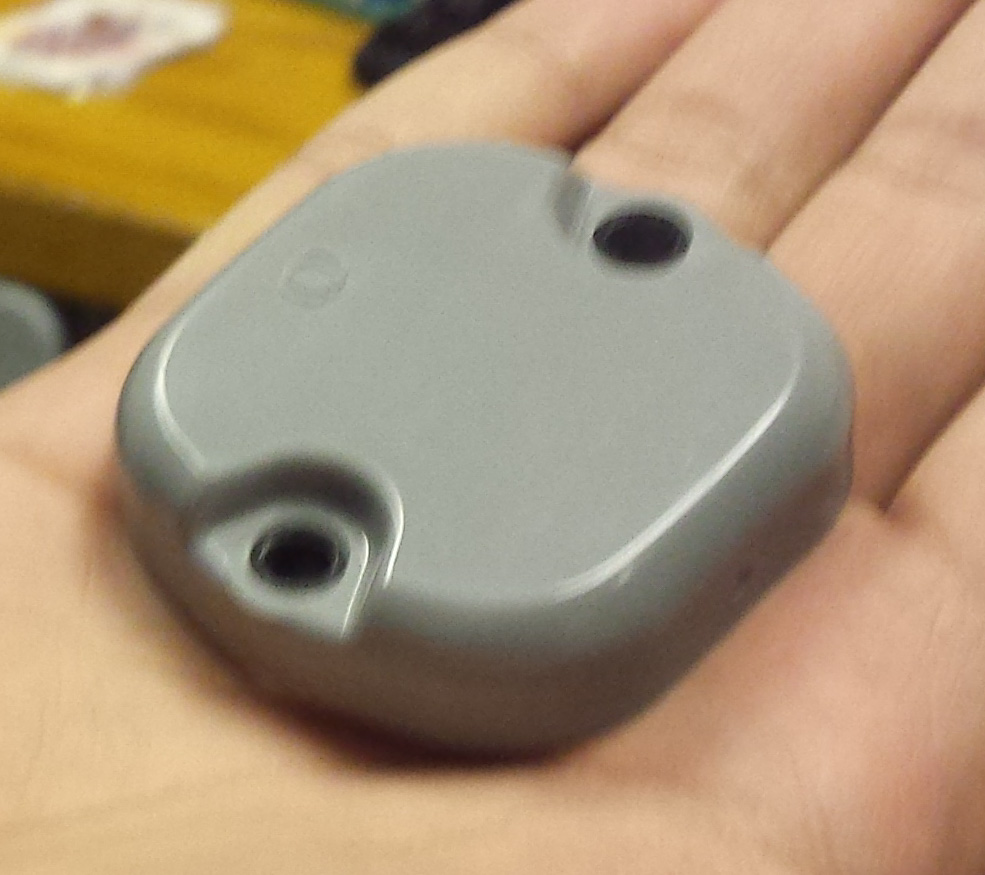
\includegraphics[scale=0.8]{img/20150429_120113_edited.jpg}}
\caption{Tested RFID tag}
\label{tag}
\end{figure}
%%%%%
\subsection{Software}
The implementation of the software was mainly done in C\# using Visual Studio. The components of the software consists of the front-end and the back-end logic. These components communicate with each other using SQL database.
\subsubsection{Back-end logic}
In order to connect to the RFID readers a script was developed by the team in C\#. This Script connects to the reader and sends a command that asks the reader about any tag in the range. The following code establishes the connection and starts an infinite loop to keep reading the tags using another method until the process is manually canceled:
\lstset{style=sharpc}
\begin{lstlisting}
 string hostName = "172.16.10.99";
 int hostPort = 50007;

 IPAddress host = IPAddress.Parse(hostName);
 IPEndPoint hostep = new IPEndPoint(host, hostPort);
 Socket socket = new Socket(AddressFamily.InterNetwork, SocketType.Stream, ProtocolType.IP);
 while (!socket.Connected){
  socket.Connect(hostep);
 }
 while (true){
  try{
    NetworkStream nw = new NetworkStream(socket);
    sw = new StreamWriter(nw);
    sr = new StreamReader(nw);
    Tag[] tags = readTags();
  }
  catch (Exception){
    Console.WriteLine("something went wrong");
  }
\end{lstlisting}
The following method is the method that is responsible of sending the read command to the reader, when it fitches the tags it will check for the "ok" string to make sure that there are tags detected, if tags were detected it will start splitting the information and assign the values received into a custom type called "Tag".
\lstset{style=sharpc}
\begin{lstlisting}
 static Tag[] readTags(){ 
  string command = "tag.db.scan_tags(100)";
  writeCommand(command);
  Tag[] tags = new Tag[15];

  if (sr.ReadLine().Equals("ok")){
   char[] delimiterChars = { '=', ',' };
   int i = 0;
   string[] words;
   while ((words = sr.ReadLine().Split(delimiterChars)).
                      Length != 1){
    tags[i] = new Tag();
    tags[i].id = words[1];
    tags[i].readTime = DateTime.Parse(words[5]).TimeOfDay;
    tags[i].antenna = Int32.Parse(words[9]);
    var x = tags[i].id;
    int antenna = tags[i].antenna;
\end{lstlisting}
After that the code will write the new data to the database using MS SQL connection string.

\subsubsection{SQL database} The database was implemented in MS SQL. In \figref{sql} it shows the tables and their columns.\\
\begin{figure}[ht]
\centering
\fbox{add the sql SS}
\caption{MS SQL environment}
\label{sql}
\end{figure}
\subsubsection{Front-end implementation}
The front-end was implemented using the ASP.NET webforms technology. This technology minimized the development time and provided a consistent web application with the benefit of flexibility and compatibility with C\# code. The interface developed is shown in \figref{web}.
\begin{figure}
\centering
\fbox{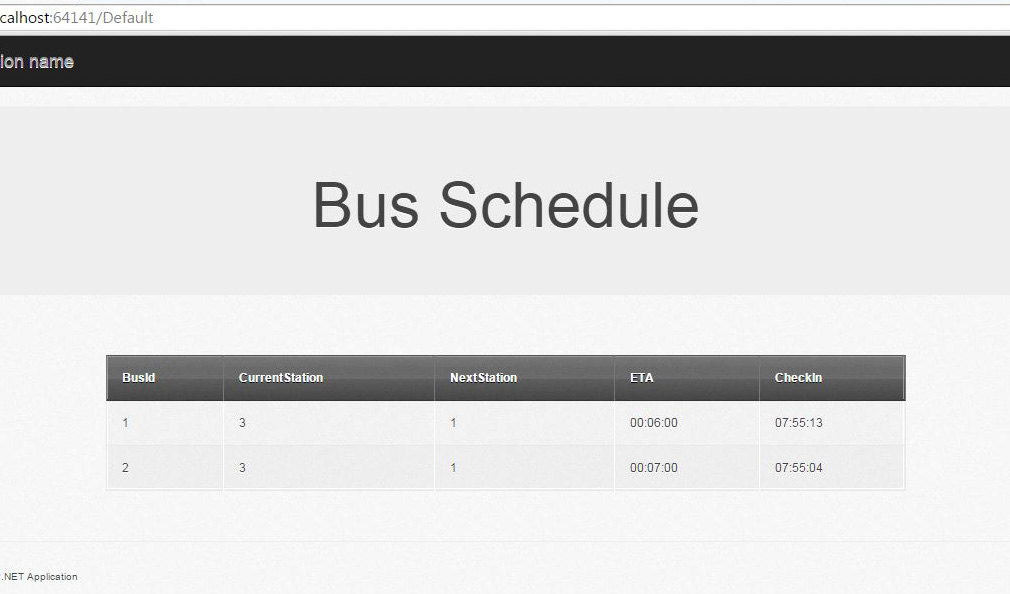
\includegraphics{img/web.jpg}}
\caption{Web interface}
\label{web}
\end{figure}


%%%%%%%%%
%%%%%%%%%
\section{Discussion}
The project has been tested by applying some scenarios to simulate the real life application. Some of these scenarios were applied on a real size car and on the run with speed that is close to the real speed of the busses. some of the tests aimed to test the system and its functionality. Although the system worked fine still there were some challenges and there is still some limitations.
%%%%
\subsection{Challenges}
The main challenge that was faced by the team is the interference and reflections by the metal objects and parts in the car and the field of the test. This challenge was solved by placing the tag on the top of the car and orient the antenna horizontally with a slight angle up word. Another challenge was the limited tools and softwares by the company, in order to overcome this issue we had to develop our own tools. In case this project is planned to be deployed, a new tools and well documented hardware should be used.
%%%%
\\

This project can be further developed since the RFID technology will never stop growing. In future work, the system may install more reliable antennas that can detect the busses from further distances and it can cover more areas for the busses.

%%%%%%%%
%%%%%%%%
\section{Conclusion}
In conclusion, RFID technology is not a new technology, although it is still growing. This application is just a small example about what RFID technology is capable to do. Applying RFID applications is not a hard task to accomplish and the results are always pleasing. This project has motivated us as a team to learn more about how RFID communication systems are implemented and what capabilities it has.




\bibliographystyle{ieeetran}
\bibliography{bib}


\end{document}


